\documentclass[a4paper,11pt]{article}
\usepackage{amsmath,amsthm,amsfonts,amssymb,amscd,amstext,vmargin,graphics,graphicx,tabularx,multicol} \usepackage[french]{babel}
\usepackage[utf8]{inputenc}  
\usepackage[T1]{fontenc} 
\usepackage[T1]{fontenc}
\usepackage{amsmath,amssymb}
\usepackage{pstricks-add,tikz,tkz-tab,variations}
\usepackage[autolanguage,np]{numprint} 

\setmarginsrb{1.5cm}{0.5cm}{1cm}{0.5cm}{0cm}{0cm}{0cm}{0cm} %Gauche, haut, droite, haut
\newcounter{numexo}
\newcommand{\exo}[1]{\stepcounter{numexo}\noindent{\bf Exercice~\thenumexo} : \marginpar{\hfill /#1}}
\reversemarginpar


\newcounter{enumtabi}
\newcounter{enumtaba}
\newcommand{\q}{\stepcounter{enumtabi} \theenumtabi.  }
\newcommand{\qa}{\stepcounter{enumtaba} (\alph{enumtaba}) }
\newcommand{\initq}{\setcounter{enumtabi}{0}}
\newcommand{\initqa}{\setcounter{enumtaba}{0}}

\newcommand{\be}{\begin{enumerate}}
\newcommand{\ee}{\end{enumerate}}
\newcommand{\bi}{\begin{itemize}}
\newcommand{\ei}{\end{itemize}}
\newcommand{\bp}{\begin{pspicture*}}
\newcommand{\ep}{\end{pspicture*}}
\newcommand{\bt}{\begin{tabular}}
\newcommand{\et}{\end{tabular}}
\renewcommand{\tabularxcolumn}[1]{>{\centering}m{#1}} %(colonne m{} centrée, au lieu de p par défault) 
\newcommand{\tnl}{\tabularnewline}

\newcommand{\trait}{\noindent \rule{\linewidth}{0.2mm}}
\newcommand{\hs}[1]{\hspace{#1}}
\newcommand{\vs}[1]{\vspace{#1}}

\newcommand{\N}{\mathbb{N}}
\newcommand{\Z}{\mathbb{Z}}
\newcommand{\R}{\mathbb{R}}
\newcommand{\C}{\mathbb{C}}
\newcommand{\Dcal}{\mathcal{D}}
\newcommand{\Ccal}{\mathcal{C}}
\newcommand{\mc}{\mathcal}

\newcommand{\vect}[1]{\overrightarrow{#1}}
\newcommand{\ds}{\displaystyle}
\newcommand{\eq}{\quad \Leftrightarrow \quad}
\newcommand{\vecti}{\vec{\imath}}
\newcommand{\vectj}{\vec{\jmath}}
\newcommand{\Oij}{(O;\vec{\imath}, \vec{\jmath})}
\newcommand{\OIJ}{(O;I,J)}

\newcommand{\bmul}[1]{\begin{multicols}{#1}}
\newcommand{\emul}{\end{multicols}}


\newcommand{\reponse}[1][1]{%
\multido{}{#1}{\makebox[\linewidth]{\rule[0pt]{0pt}{20pt}\dotfill}
}}

\newcommand{\titre}[5] 
% #1: titre #2: haut gauche #3: bas gauche #4: haut droite #5: bas droite
{
\noindent #2 \hfill #4 \\
#3 \hfill #5

\vspace{-1.6cm}

\begin{center}\rule{6cm}{0.5mm}\end{center}
\vspace{0.2cm}
\begin{center}{\large{\textbf{#1}}}\end{center}
\begin{center}\rule{6cm}{0.5mm}\end{center}
}



\begin{document}
\pagestyle{empty}
\titre{Interrogation sur les fractions}{Nom :}{Prénom :}{Classe}{Date}



\exo{6.5}

Calculer les expressions suivantes en détaillant toutes vos étapes de calculs et \textbf{simplifier les résultats si besoin} :

\bmul{4}

$R = \dfrac{6}{5} + \dfrac{18}{5} + \dfrac{21}{5}$\\
\reponse[5]\\


\columnbreak

$E = \dfrac{5}{3} - \dfrac{10}{12}$\\ 
\reponse[5]\\

\columnbreak

$P = 3 - \dfrac{2}{7}$\\ 
\reponse[5]\\

\columnbreak

$S =\dfrac{1}{3}+\dfrac{4}{5} - \dfrac{11}{45}$\\ 
\reponse[5]\\

\emul

\bmul{2}

$F = \dfrac{21}{4} - \left( \dfrac{1}{2} - \dfrac{1}{4}   \right)$\\ 
\reponse[6]\\

\columnbreak

$M = \left(  \dfrac{7}{6}+\dfrac{2}{3} \right)- \left(\dfrac{11}{9} + \dfrac{7}{18}\right)$\\ 
\reponse[6]\\

\emul


\vspace*{0.6cm}

\exo{2}

Dans une carafe d'un litre, on mélange $\dfrac{1}{2}$ L de jus d'orange, $\dfrac{1}{20}$ L de jus de citron, $\dfrac{1}{10}$ L de jus de pamplemousse et $\dfrac{2}{5}$ L de sucre de canne.\\

Quelle quantité de boisson obtient-on ? La carafe va-t-elle déborder ? Pourquoi ? (\textbf{Justifier votre réponse par des calculs.)}\\
\reponse[7]\\

\vspace*{0.5cm}

\newpage

\exo{1,5} Compléter la pyramide ci-dessous, de façon à ce que chaque case soit la somme des cases situées juste en dessous. Écrire vos calculs juste en dessous.\\

\begin{center}

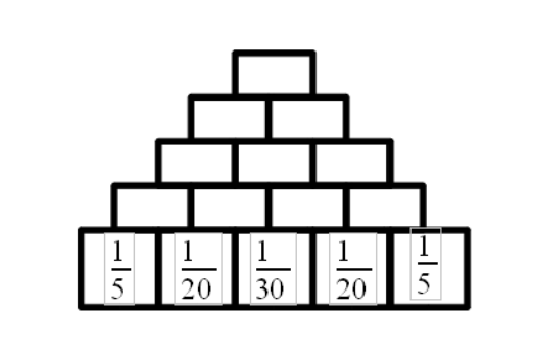
\includegraphics[scale=1.1]{pyramide.eps} 
\end{center}

\reponse[8]


\end{document}
